\documentclass[border=6pt,tikz]{standalone}
\usepackage{tikz}
\usepackage{amsmath,amssymb}
\usetikzlibrary{arrows.meta,positioning,fit,backgrounds,calc,shapes.geometric,decorations.pathreplacing,patterns}
\definecolor{ink}{HTML}{1B2430}
\definecolor{muted}{HTML}{6B7785}
\definecolor{accent}{HTML}{2F6FB5}
\definecolor{accent2}{HTML}{C1611F}
\definecolor{good}{HTML}{2E7D5B}
\definecolor{soft}{HTML}{EDF2F7}
\definecolor{soft2}{HTML}{FBEDE2}
\definecolor{soft3}{HTML}{E6F0E9}
\tikzset{
  box/.style={draw=ink,line width=.7pt,rounded corners=2pt,fill=soft,inner sep=4pt,align=center,font=\sffamily\small},
  boxa/.style={box,fill=soft2},
  boxb/.style={box,fill=soft3},
  plain/.style={align=center,font=\sffamily\small,text=ink},
  tiny/.style={align=center,font=\sffamily\scriptsize,text=muted},
  ar/.style={-{Stealth[length=2.4mm]},draw=ink,line width=.7pt},
  arm/.style={-{Stealth[length=2.4mm]},draw=muted,line width=.6pt,dashed},
  nd/.style={circle,draw=ink,line width=.7pt,fill=white,minimum size=7mm,inner sep=0pt,font=\sffamily\scriptsize},
  ndf/.style={nd,fill=soft},
  ndt/.style={nd,fill=soft2},
}

\begin{document}
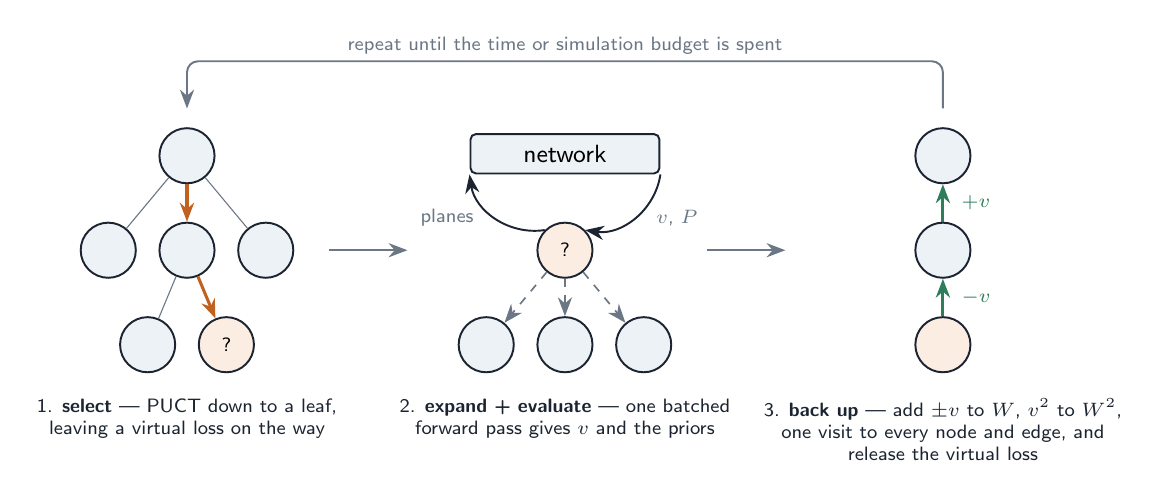
\begin{tikzpicture}[x=1mm,y=1mm]
  % ── 1. select ──
  \begin{scope}[shift={(0,0)}]
    \node[ndf] (r) at (16,32) {};
    \node[ndf] (a) at (6,20) {}; \node[ndf] (b) at (16,20) {}; \node[ndf] (c) at (26,20) {};
    \node[ndf] (d) at (11,8) {}; \node[nd,fill=soft2] (e) at (21,8) {?};
    \draw[draw=muted] (r)--(a) (r)--(c) (b)--(d);
    \draw[ar,draw=accent2,line width=1.1pt] (r)--(b); \draw[ar,draw=accent2,line width=1.1pt] (b)--(e);
    \node[tiny,text=ink,below=2mm of e.south,xshift=-5mm] {1. \textbf{select} --- PUCT down to a leaf,\\leaving a virtual loss on the way};
  \end{scope}
  % ── 2. expand+evaluate ──
  \begin{scope}[shift={(48,0)}]
    \node[nd,fill=soft2] (e2) at (16,20) {?};
    \node[box,above=6mm of e2,minimum width=24mm] (nn) {network};
    \node[ndf] (f) at (6,8) {}; \node[ndf] (g) at (16,8) {}; \node[ndf] (h) at (26,8) {};
    \draw[arm] (e2)--(f); \draw[arm] (e2)--(g); \draw[arm] (e2)--(h);
    \draw[ar] (e2.north west) to[bend left=45] node[tiny,left,xshift=-1.5mm]{planes} (nn.south west);
    \draw[ar] (nn.south east) to[bend left=45] node[tiny,right,xshift=1.5mm]{$v$, $P$} (e2.north east);
    \node[tiny,text=ink,below=2mm of g.south] {2. \textbf{expand + evaluate} --- one batched\\forward pass gives $v$ and the priors};
  \end{scope}
  % ── 3. backup ──
  \begin{scope}[shift={(96,0)}]
    \node[ndf] (r3) at (16,32) {}; \node[ndf] (b3) at (16,20) {}; \node[ndt] (e3) at (16,8) {};
    \draw[ar,draw=good,line width=1.1pt] (e3)--node[tiny,right,text=good,xshift=1mm]{$-v$}(b3);
    \draw[ar,draw=good,line width=1.1pt] (b3)--node[tiny,right,text=good,xshift=1mm]{$+v$}(r3);
    \node[tiny,text=ink,below=2mm of e3.south] {3. \textbf{back up} --- add $\pm v$ to $W$, $v^2$ to $W^2$,\\one visit to every node and edge, and\\release the virtual loss};
  \end{scope}
  \draw[ar,draw=muted] (34,20) -- (44,20);
  \draw[ar,draw=muted] (82,20) -- (92,20);
  \draw[ar,draw=muted,rounded corners] (112,38) -- (112,44) -- (16,44) -- (16,38);
  \node[tiny] at (64,46) {repeat until the time or simulation budget is spent};
\end{tikzpicture}
\end{document}
